\selectlanguage{english}

\acresetall %supposed to have the acronyms just defined once per chapter, doesn't seem required


\chapter{Chapter: Types of section distinctions}

\begin{lstlisting}
\chapter{Chapter: Types of section distinctions}
\blindtext
\section{Section} 
\blindtext
\subsection{Subsection}
\blindtext
\subsubsection{Subsubsection}
\blindtext
\end{lstlisting}
\blindtext
\section{Section} 
\blindtext
\subsection{Subsection}
\blindtext
\subsubsection{Subsubsection}
\blindtext



\section{References and labels}



\subsection{Labels}


Make sure to label sections to refer back to throughout your work. Make it an intuitive name.
%
\begin{lstlisting}
\label{sec:cosmicrays}
\label{subsec:crs_eas}
\end{lstlisting}



\subsection{Referencing labels}

Use cref instead of ref; it smartly labels if it's a section, chapter, figure, table, etc. \cref{fig:crs_eas_heitler1}.
%
\begin{lstlisting}
\cref{fig:crs_eas_heitler1}
\cref{subsec:fd}
\end{lstlisting}



\subsection{Citations}

If you have a ton of reference, just list them with commas. Latex will properly format \cite{Abraham2009b,Abraham2009,Abraham2010a,Abraham2010,Abreu:2011zze,Abreu:2011zzd,Abreu:2011vm,Abreu:2011ki,Abreu:2011fb,Settimo:2012zz,Auger:2012yc,Auger:2012an,Acounis:2012dg,Abreu:2012zz,Abreu:2012zg,Abreu:2012ybu,Abreu:2012pi,Abreu:2012oza,Abreu:2012aniso,Abreu:2011md,Abreu:2013zbq,Abreu:2013qtw,Abreu:2013qfa,Abreu:2013kif,Abreu:2013env,Aab:2014qva,Aab:2014pza,Aab:2014kda,Aab:2014ila,Aab:2014gua,Aab:2014esa,Aab:2014dua,Aab:2014dha,Aab:2014caa,Aab:2014bha,Aab:2014aea,ThePierreAuger:2014nja,PierreAuger:2014yba,Aab2015a,Aab2015,Aab:2015kma}:
\begin{lstlisting}
\cite{Abraham2009b,Abraham2009,Abraham2010a,Abraham2010,Abreu:2011zze,Abreu:2011zzd,Abreu:2011vm,Abreu:2011ki,Abreu:2011fb,Settimo:2012zz,Auger:2012yc,Auger:2012an,Acounis:2012dg,Abreu:2012zz,Abreu:2012zg,Abreu:2012ybu,Abreu:2012pi,Abreu:2012oza,Abreu:2012aniso,Abreu:2011md,Abreu:2013zbq,Abreu:2013qtw,Abreu:2013qfa,Abreu:2013kif,Abreu:2013env,Aab:2014qva,Aab:2014pza,Aab:2014kda,Aab:2014ila,Aab:2014gua,Aab:2014esa,Aab:2014dua,Aab:2014dha,Aab:2014caa,Aab:2014bha,Aab:2014aea,ThePierreAuger:2014nja,PierreAuger:2014yba,Aab2015a,Aab2015,Aab:2015kma}
\end{lstlisting}



\section{Acronoyms}

There's a neat package called acronyms that will handle them for you. Alex had already set this in the acronym.tex. Just define your acronyms here as he did.

\begin{itemize}
\item To use the acronym like \ac{CR}, use:
\begin{lstlisting}
\ac{CR}
\end{lstlisting}
%
\item To define the acronym in the text---\acfi{CMB}, use:
\begin{lstlisting}
\acfi{CMB}
\end{lstlisting}
If you want this to be the only place in your chapter where the acronym is defined, you need to write:
\begin{lstlisting}
\acfi{CMB}\acused{CMB}
\end{lstlisting}
as the acronym package does not automatically count this as a definition.
%
\item To makes the acronym plural. CAVEAT is that acronyms ending in an S will add an extra S which is not typically used in English.
\begin{lstlisting}
\acp{CR}
\end{lstlisting}
\item Sometimes acronyms require more complicated definitions, you can define them in the main document and call them throughout. Alex has already defined \qgsjet and \Offline:
\begin{lstlisting}
 \qgsjet
 \Offline
\end{lstlisting}
\end{itemize}



\section{Units}

For defining units, use the SI package, as it will consistently format for you. It sometimes may not recognize something like Mpc.

Examples:
%
\begin{itemize}
\item \SI{e20}{\eV}
\item \SI{12}{\square\km} for multiple units
\item \SI{90}{\percent} for precentages
\item $\approx \SI{5e19}{\eV}$
\item \SI{37}{\grammage} for grammage
\item \SI{30}{\giga\eV}  if GeV is not recognized, specify by metric prefix
\item \SI{3e15}{\eV}
\item \SIrange{30}{60}{\percent} a way to consistently format ranges
\item $\si{\square\km \steradian \year}$
\end{itemize}

\begin{lstlisting}
\SI{e20}{\eV}
\SI{12}{\square\km}
\SI{90}{\percent} 
$\approx \SI{5e19}{\eV}$
\SI{37}{\grammage}
\SI{30}{\giga\eV} 
\SI{3e15}{\eV} 3{\times}10^{19}
\SIrange{30}{60}{\percent} 
$\si{\square\km \steradian \year}$
\end{lstlisting}



\section{Figures}

In a PhD thesis you should always use only \verb![t]! (top) figure placement. Also note that due to the \verb!\graphicspath{{figures/}}! command in the preamble, the file paths are relative to the \verb!./figures! directory which can thus be dropped from the line. If you also ommit the filename extension (e.g.\ \verb!.pdf! or \verb!.jpg!) your source file will be compilable with both, \verb!latex! and \verb!pdflatex!.

\begin{figure}[t]
  \centering
  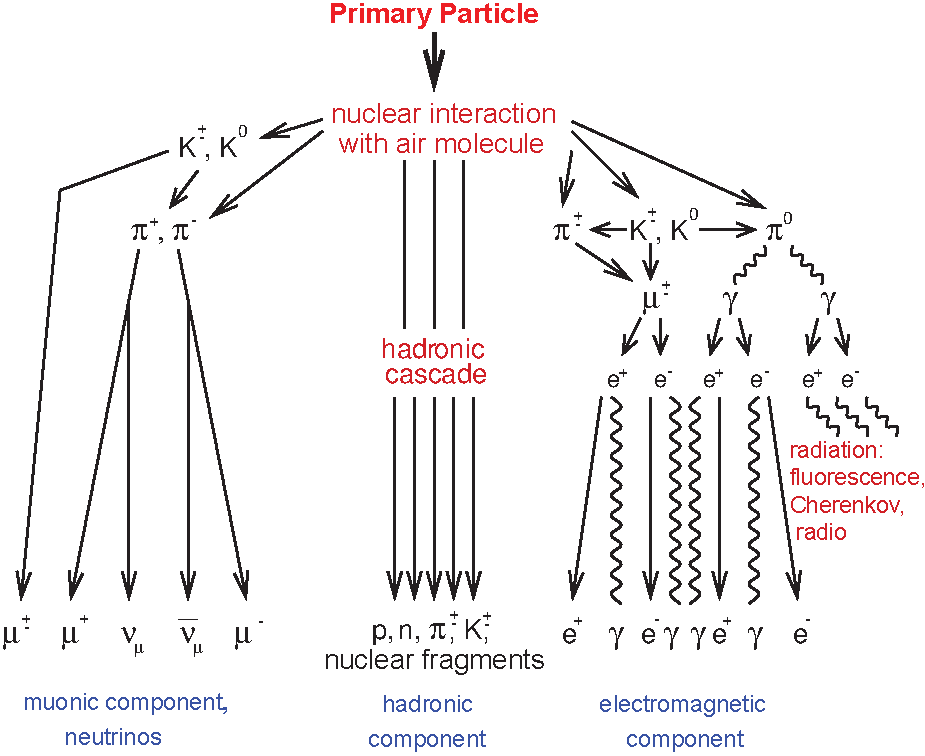
\includegraphics[width=0.8\textwidth]{intro/heitler}
  \caption{Illustration of an \ac{EAS}' particle components.}
  \label{fig:crs_eas_heitler1}
\end{figure}
\begin{lstlisting}
\begin{figure}[h]
  \centering
  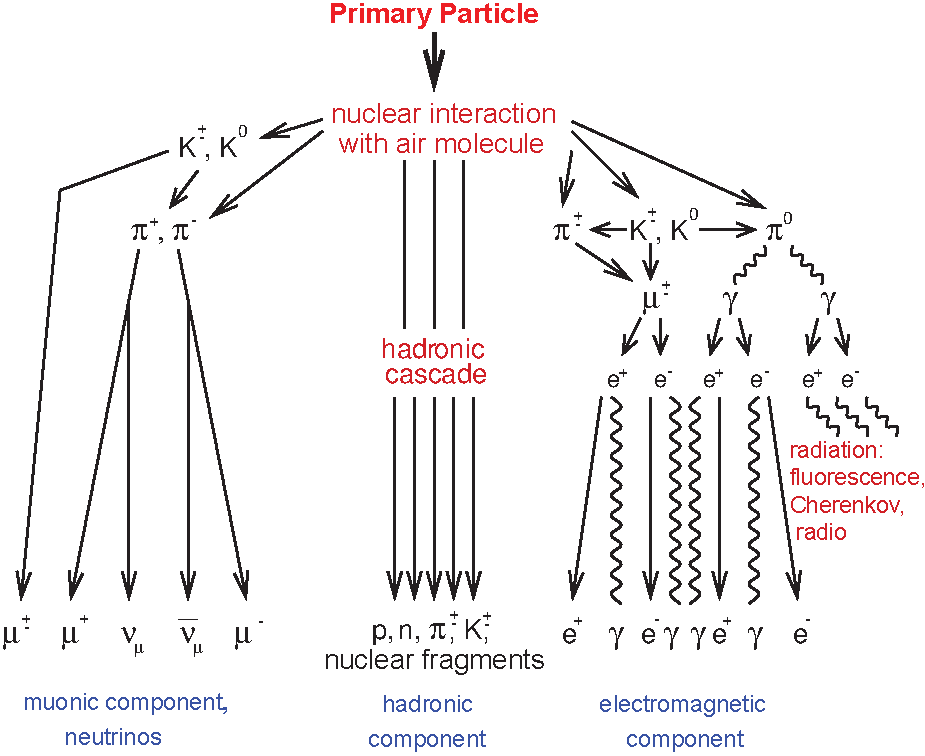
\includegraphics[width=0.8\textwidth]{intro/heitler}
  \caption{Illustration of an \ac{EAS}' particle components.}
  \label{fig:crs_eas_heitler1}
\end{figure}
\end{lstlisting}
\newpage

Use \verb!subref! to reference elements within a figure for your text or captions. 

\begin{figure}[t]
  \centering
  \subfloat[]{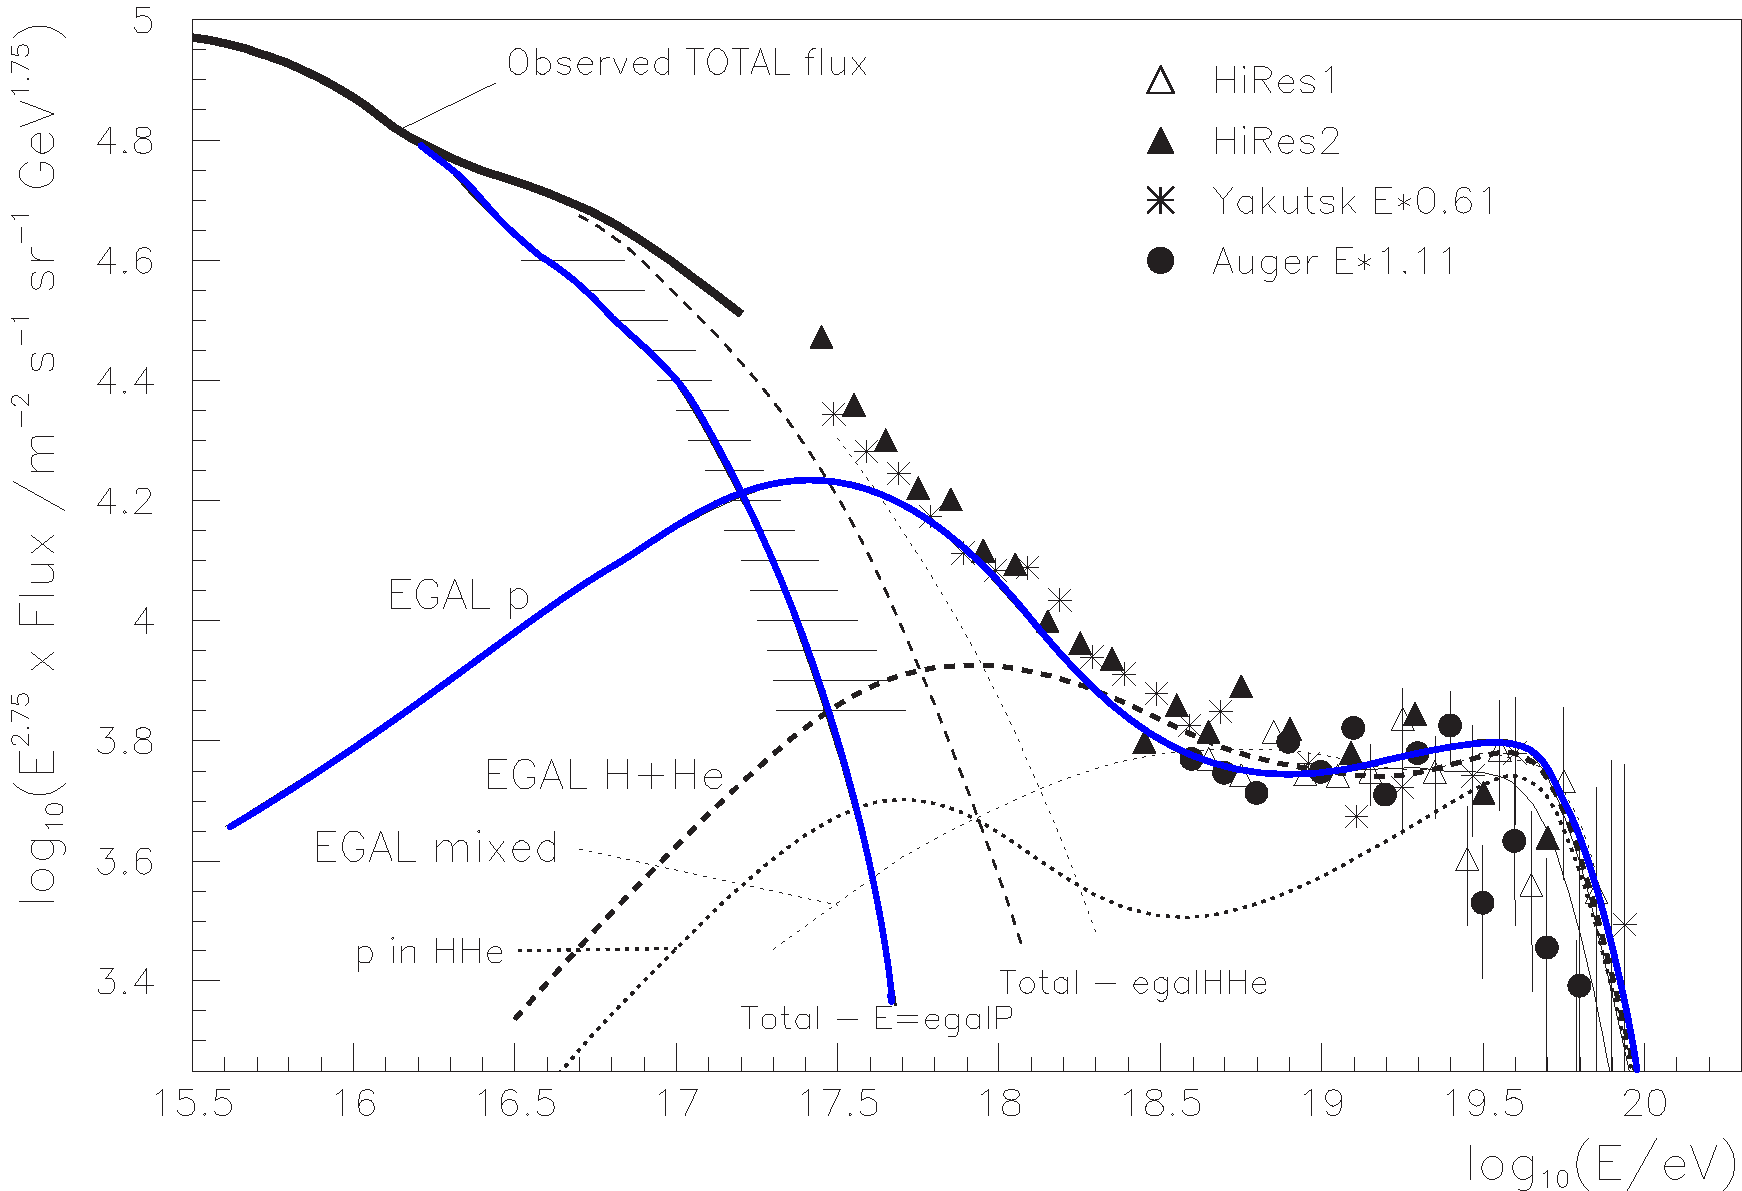
\includegraphics[width=0.48\textwidth]{intro/Berezinsky2}
  \label{plot:crs_ankle_berezinsky}
  }\hspace{0.2cm}
  \subfloat[]{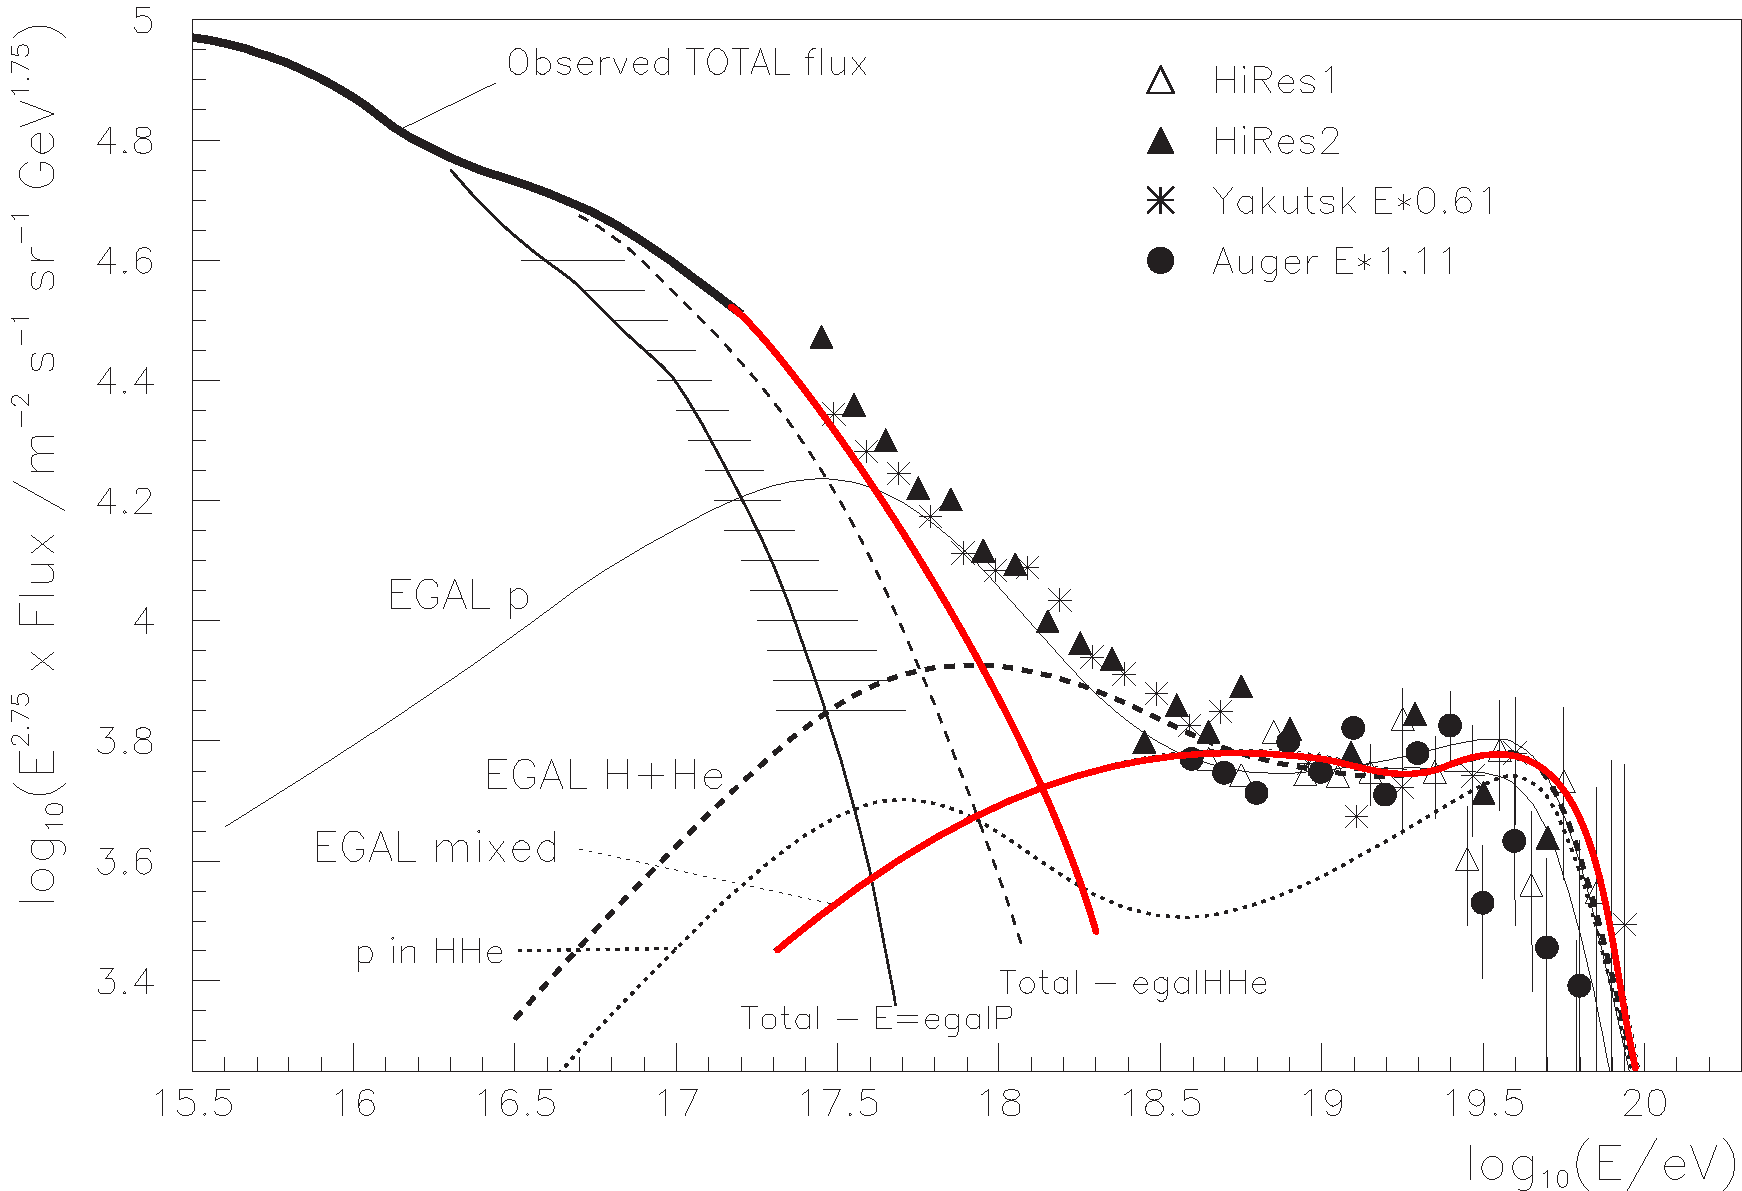
\includegraphics[width=0.48\textwidth]{intro/Hillas2}
  \label{plot:crs_ankle_hillas}
  }
  \caption[]{Visualization of the \subref{plot:crs_ankle_berezinsky} pair production dip \cite{berezinskycr} and \subref{plot:crs_ankle_hillas} mixed composition \cite{hillascr} scenarios that describe the ankle feature.}
  \label{fig:crs_ankle}
\end{figure}
\begin{lstlisting}
\begin{figure}[t]
  \centering
  \subfloat[]{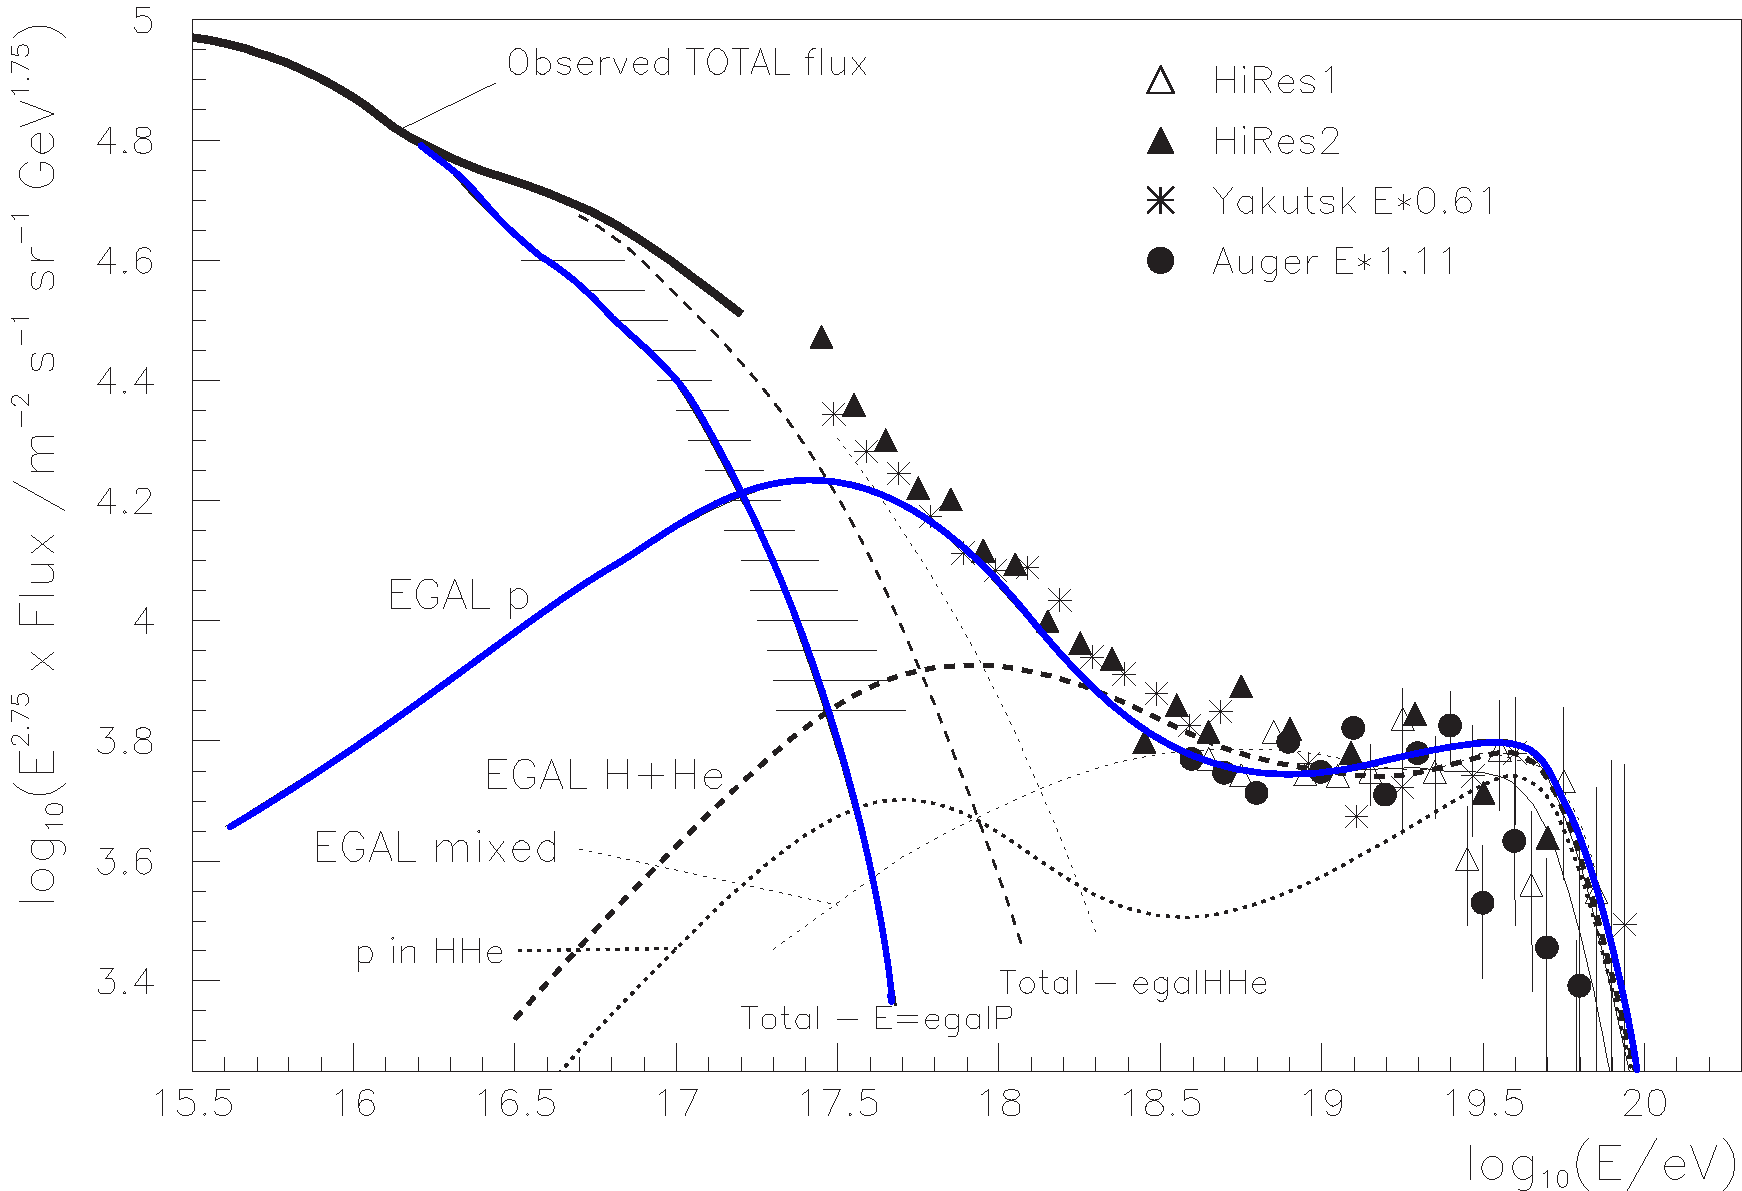
\includegraphics[width=0.48\textwidth]{intro/Berezinsky2}
  \label{plot:crs_ankle_berezinsky}
  }\hspace{0.2cm}
  \subfloat[]{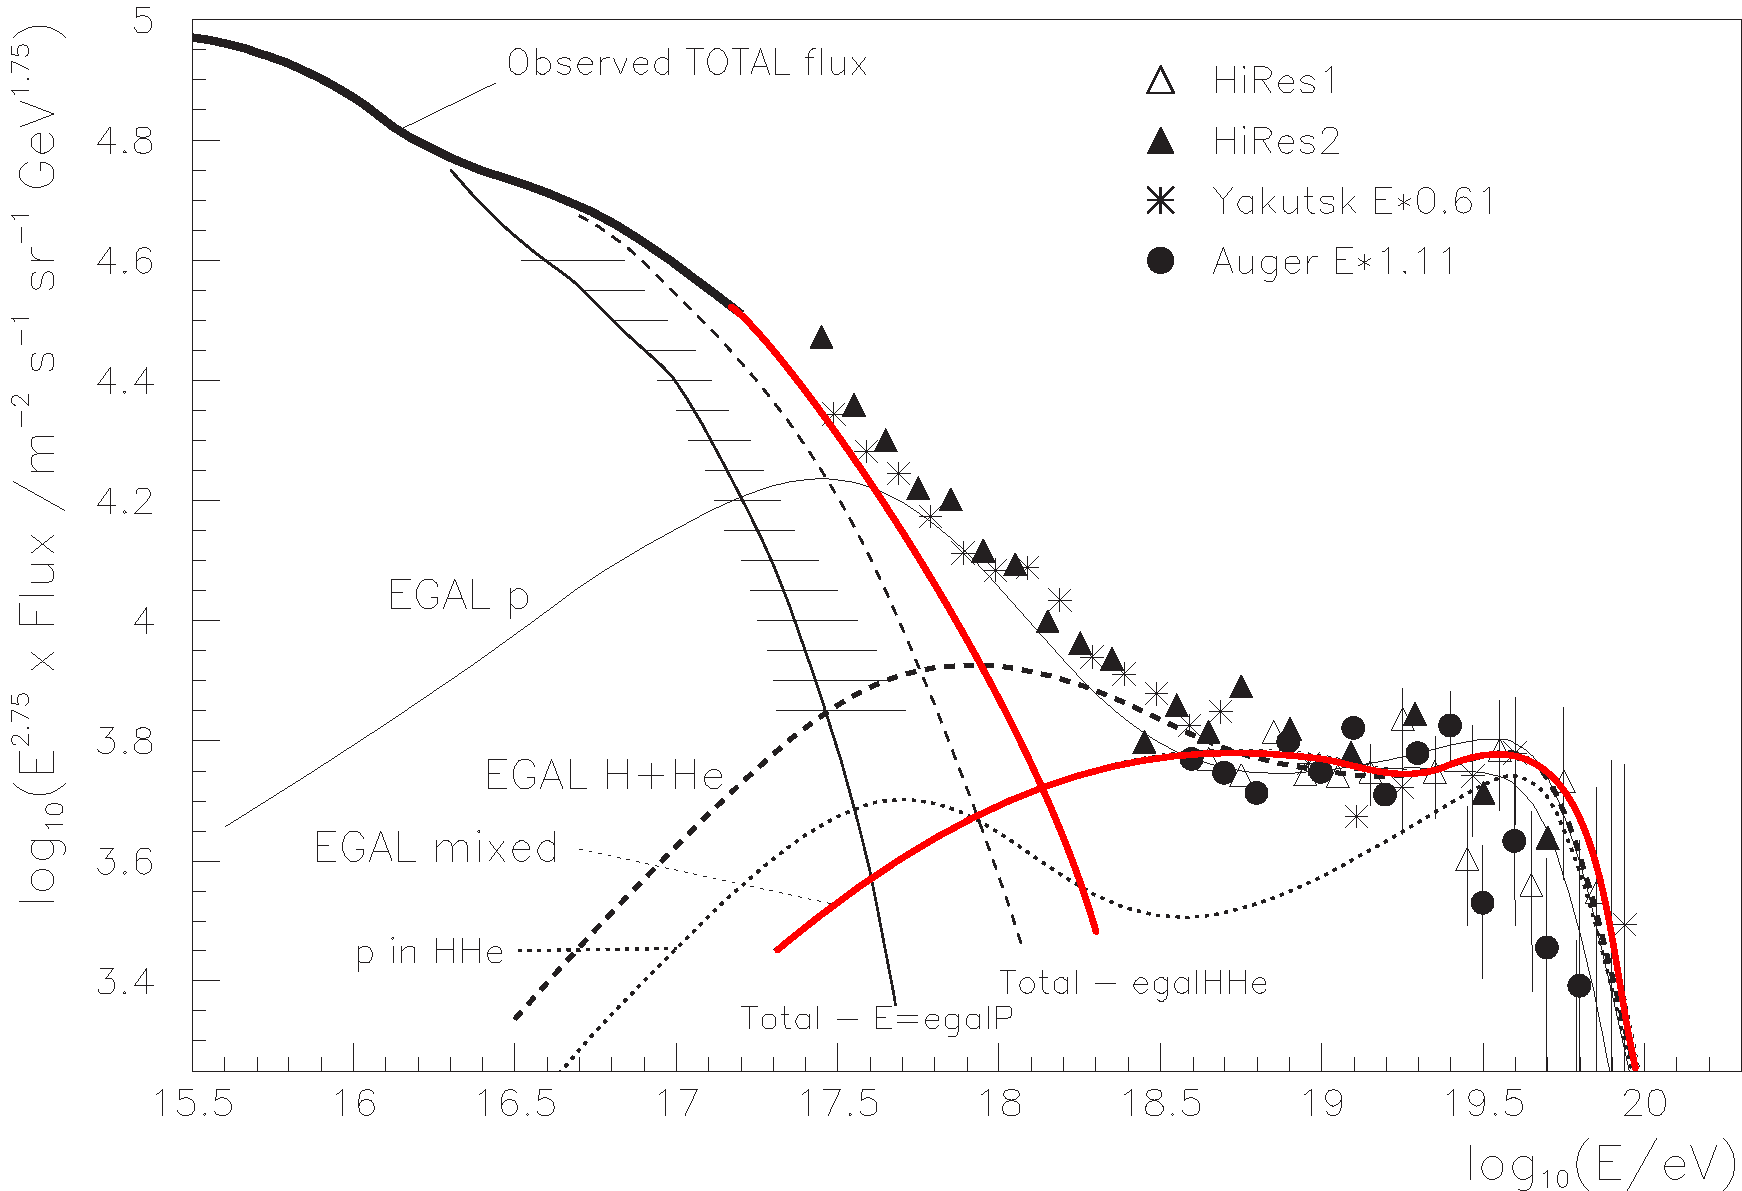
\includegraphics[width=0.48\textwidth]{intro/Hillas2}
  \label{plot:crs_ankle_hillas}
  }
  \caption[]{Visualization of the \subref{plot:crs_ankle_berezinsky} pair production dip \cite{berezinskycr} and \subref{plot:crs_ankle_hillas} mixed composition \cite{hillascr} scenarios that describe the ankle feature.}
  \label{fig:crs_ankle}
\end{figure}
\end{lstlisting}

If you need a footnote in a figure, you have to use \verb!footnotemark!
%
\begin{figure}[t]
  \centering
  \subfloat[]{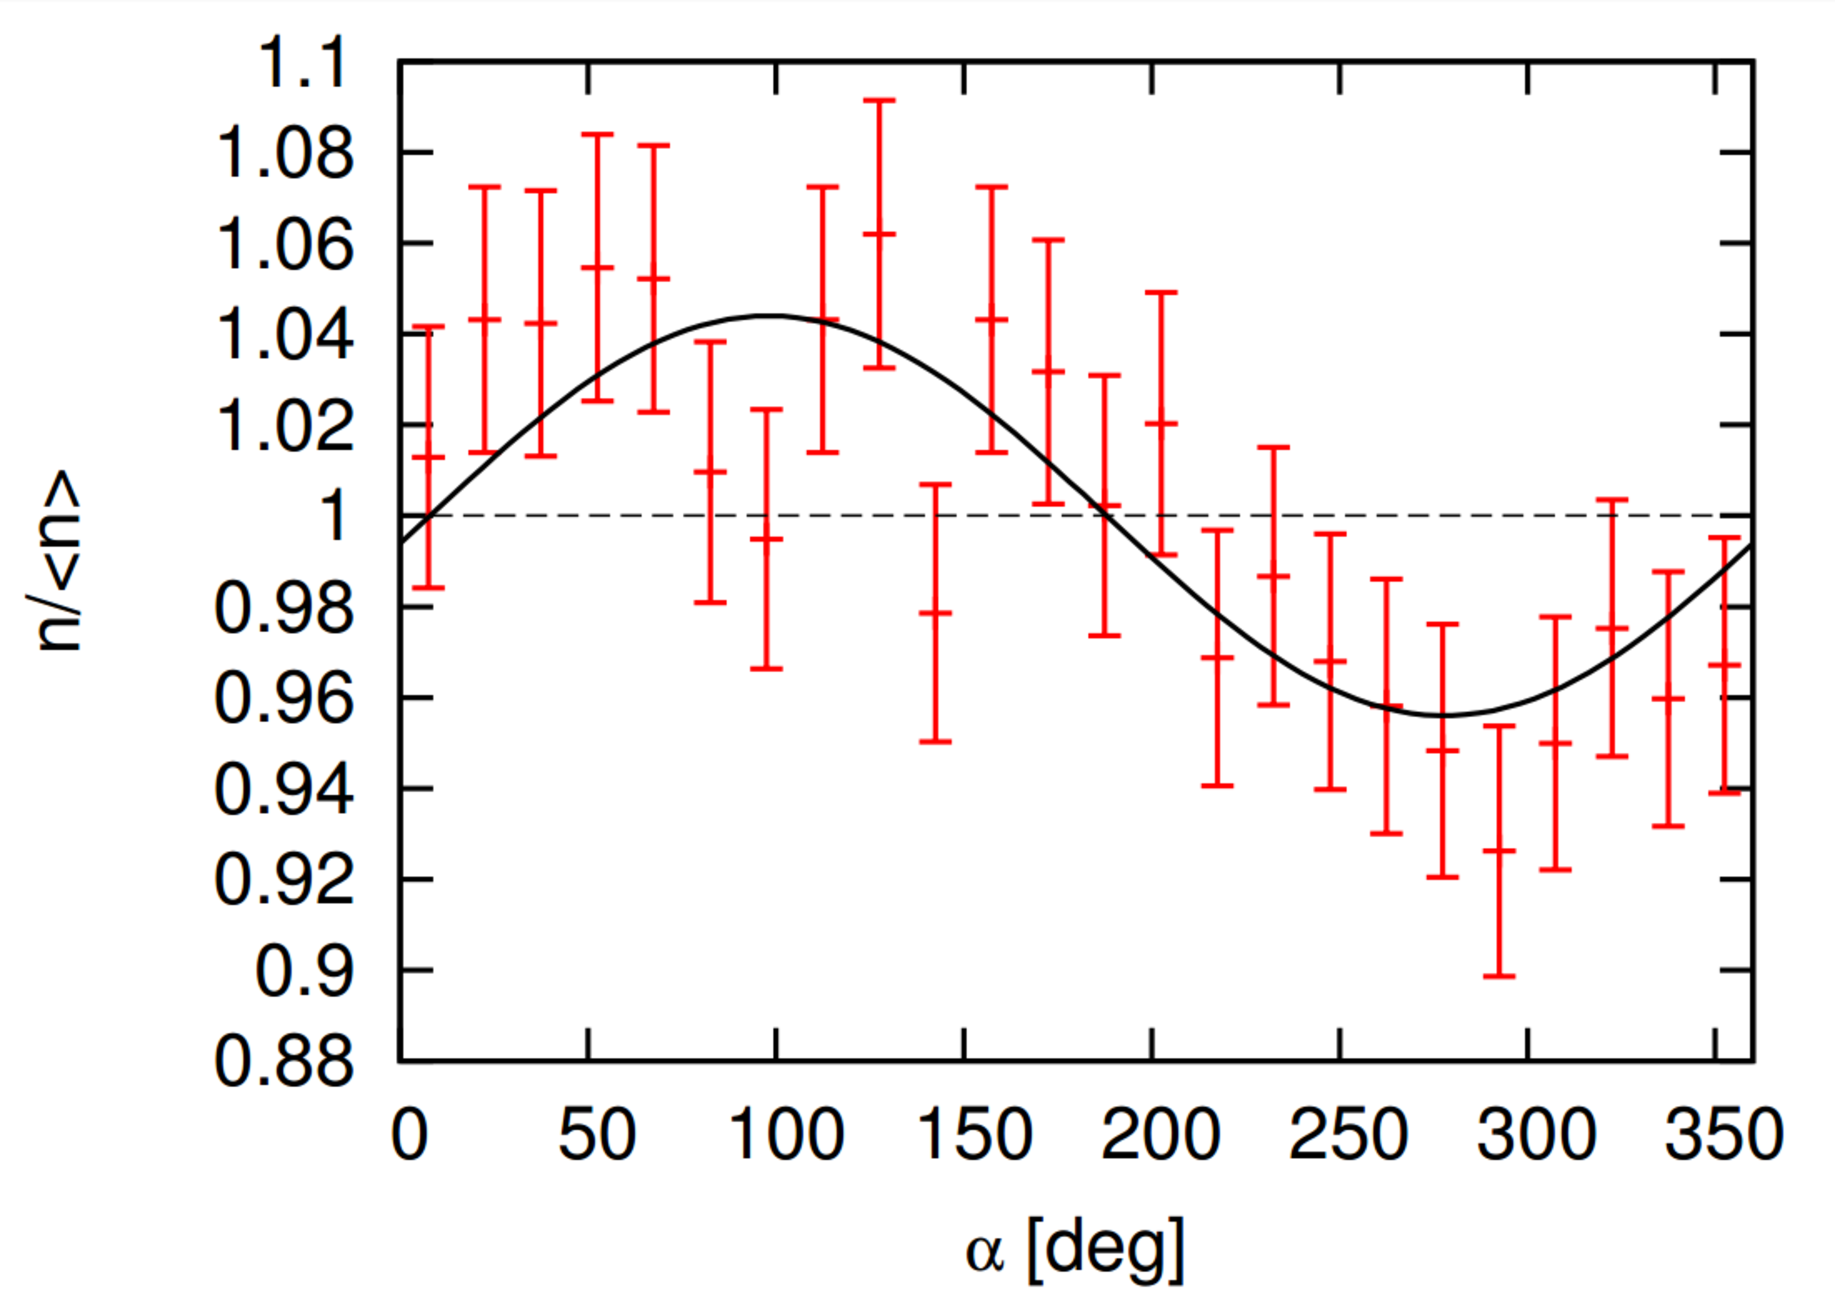
\includegraphics[height=5cm]{intro/auger_dipole}
  \label{plot:pao_dipole}}
  \subfloat[]{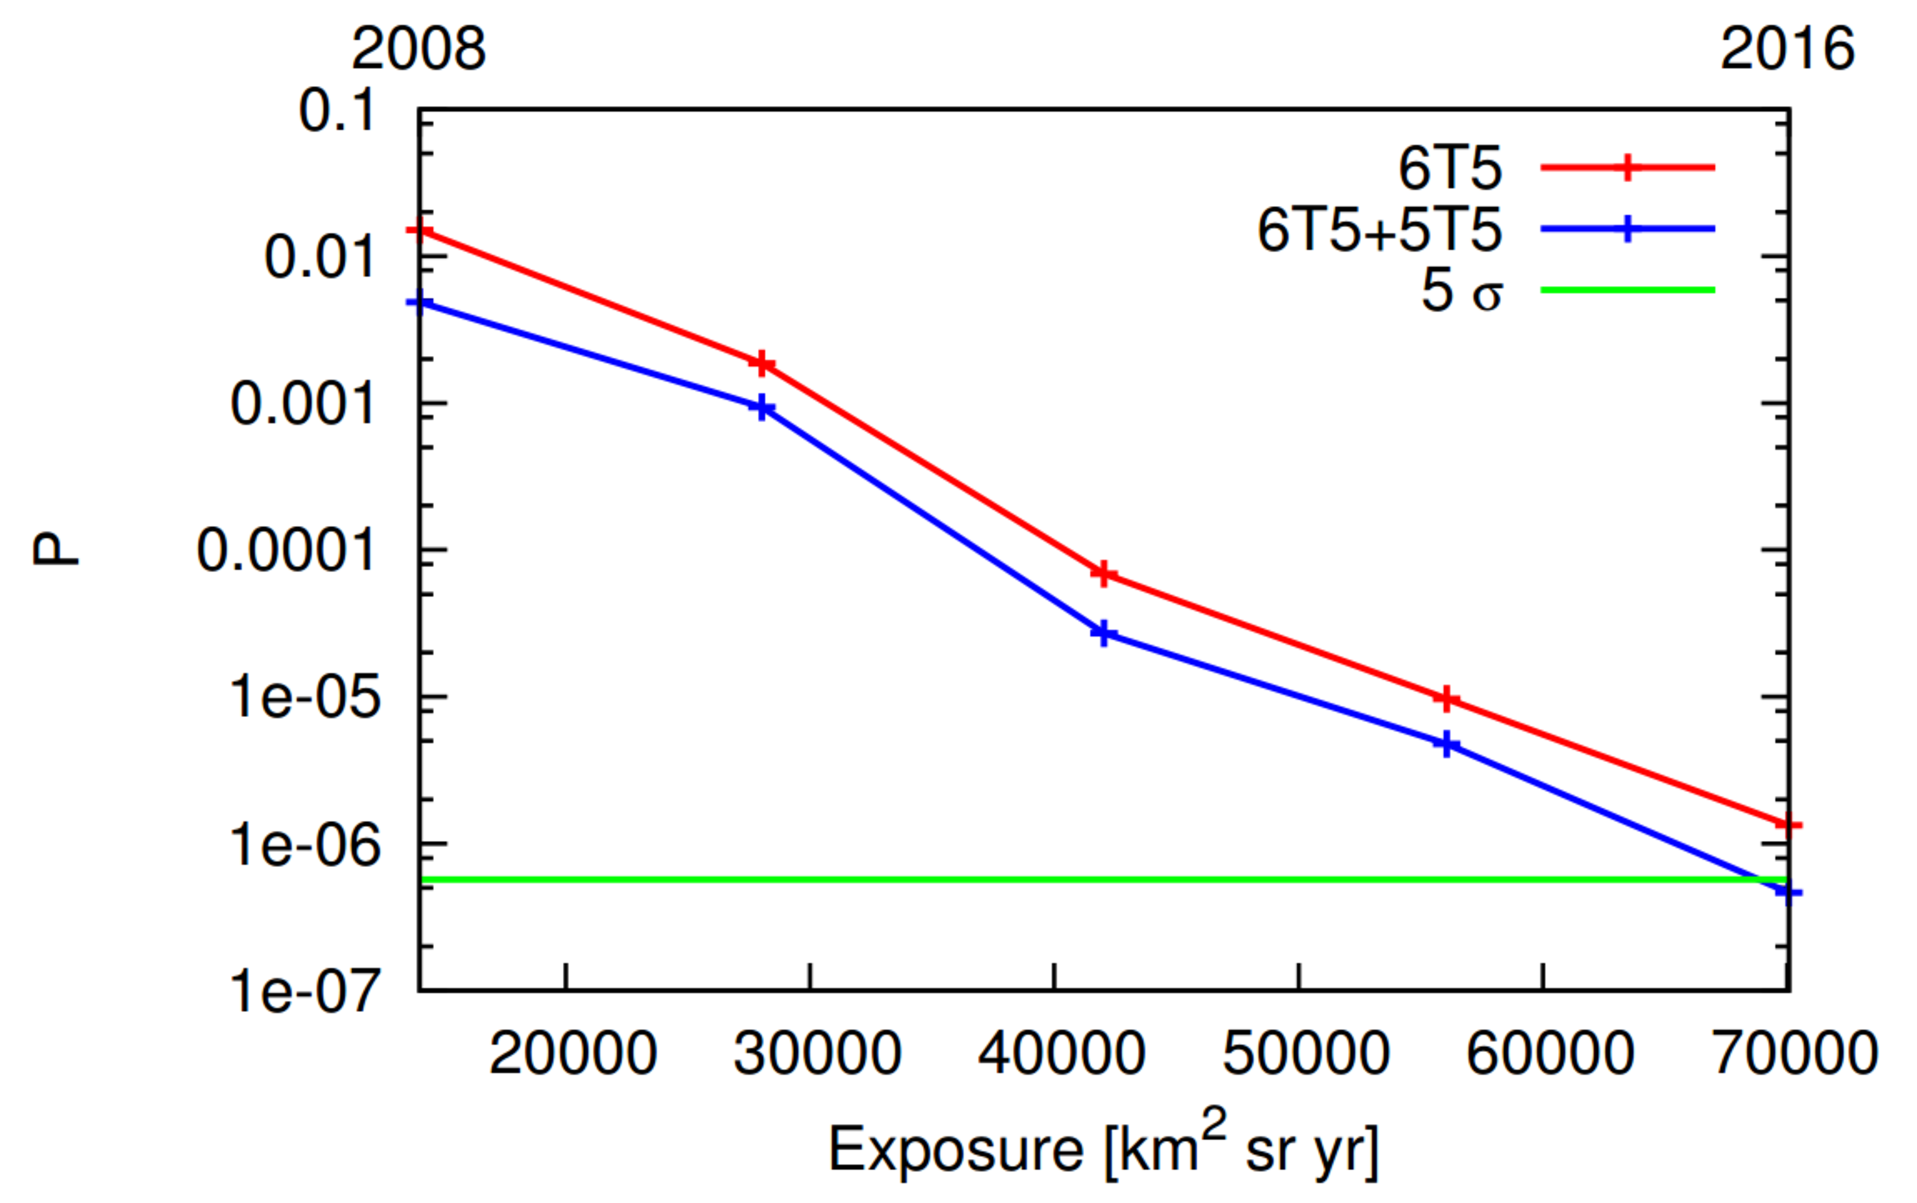
\includegraphics[height=5cm]{intro/auger_dipole_sig}
  \label{plot:pao_dipole_sig}}
  \caption[]{\subref{plot:pao_dipole} \subref{plot:pao_dipole_sig} Probability for the amplitude of the dipole to arise from an isotropic distribution as a function of the integrated exposure of the Pierre Auger Observatory. Various data sets with different tank triggers are shown \footnotemark \cite{Mollerach2016_1}.
  }
\label{fig:pao_dipole}
\end{figure}
\footnotetext{As discussed further in the reconstruction Chapter, quality cuts are performed on reconstructed data from the \ac{SD}. One of these cuts is known as the 6T5-trigger; it requires that the detector with the highest signal has all of its 6 closest neighbors working at the time of the event. Similarly, a 5T5 only requires 5 of the closest neighbors to be working.}
\begin{lstlisting}
\begin{figure}[t]
  \centering
  \subfloat[]{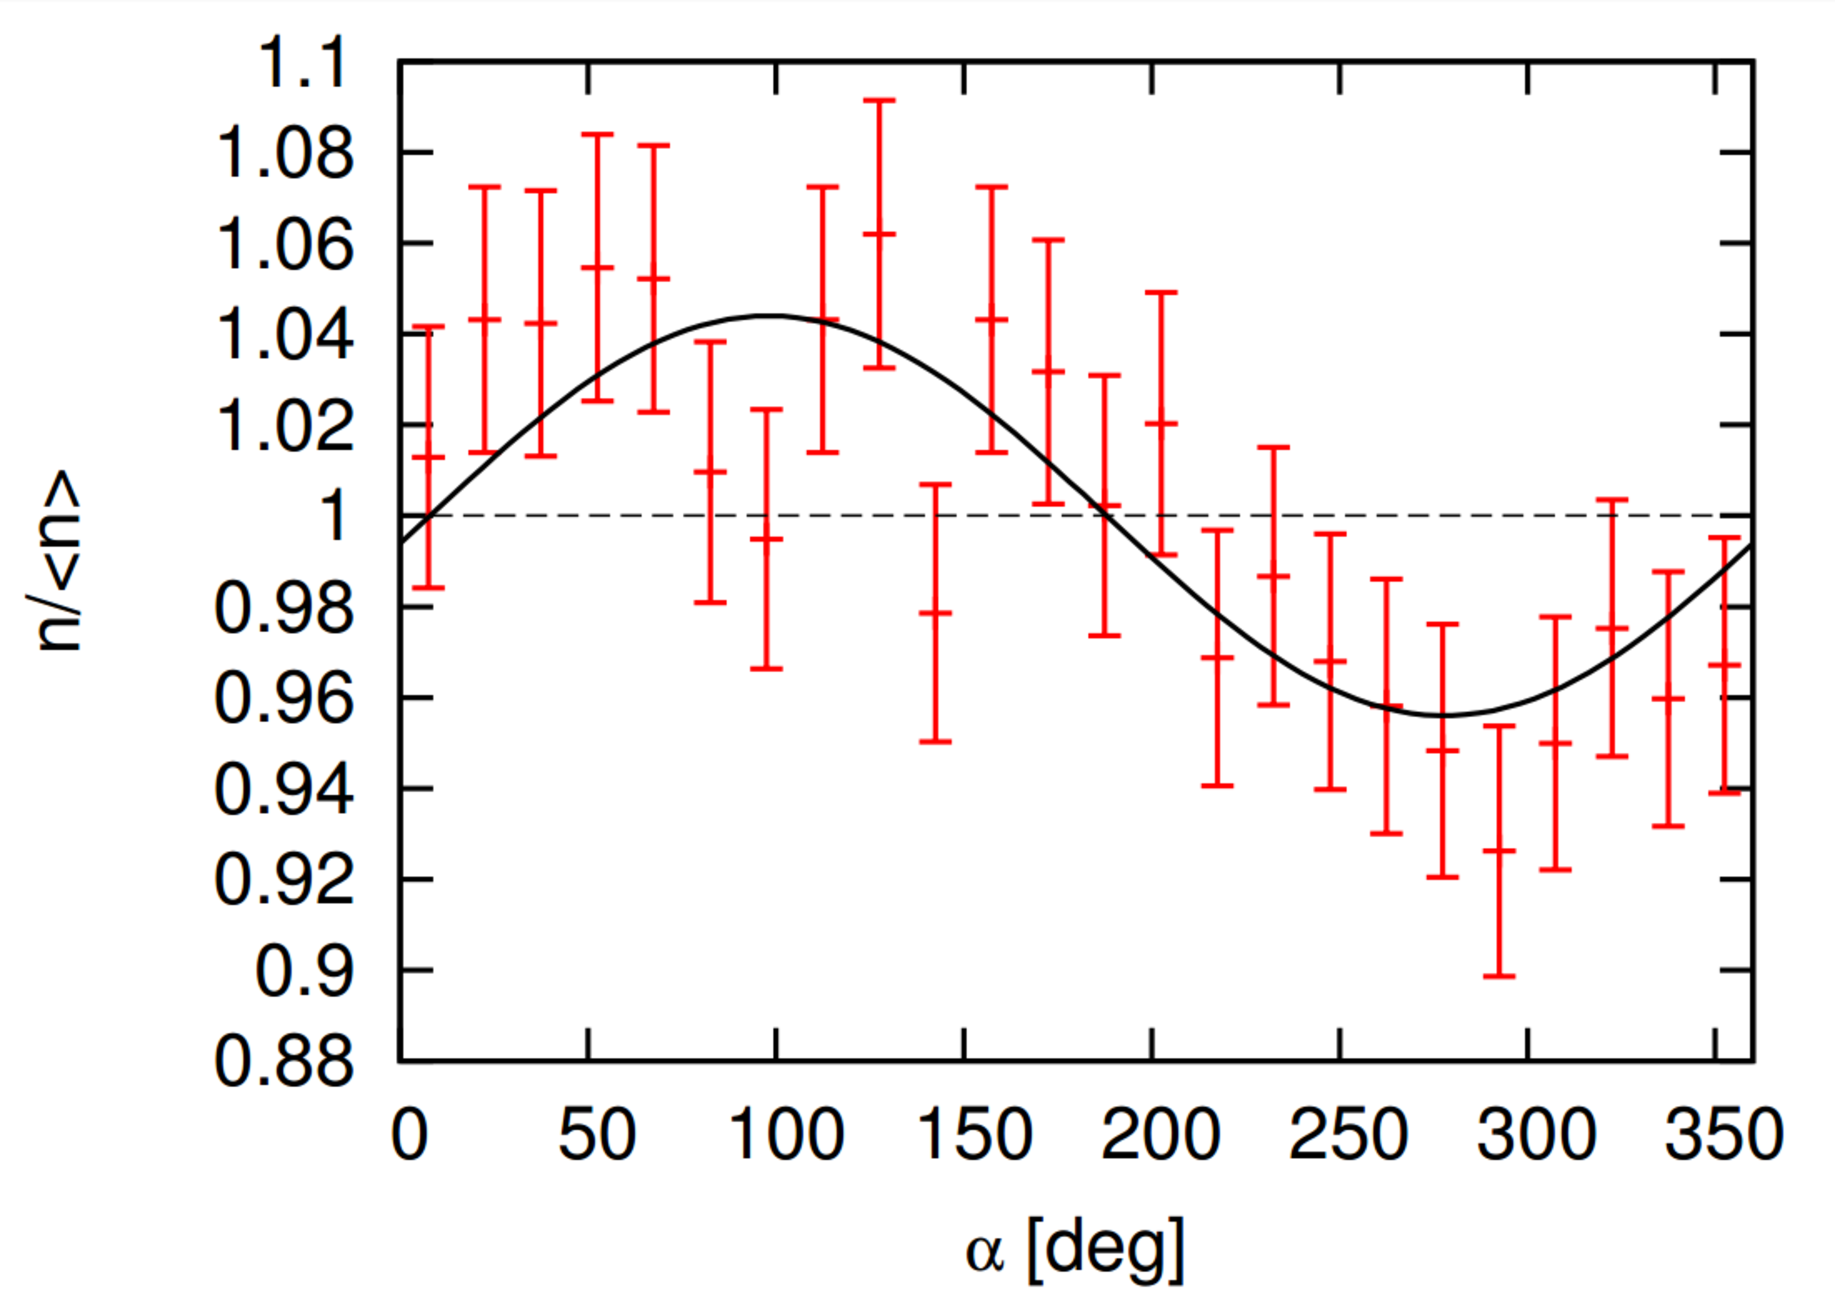
\includegraphics[height=5cm]{intro/auger_dipole}
  \label{plot:pao_dipole}}
  \subfloat[]{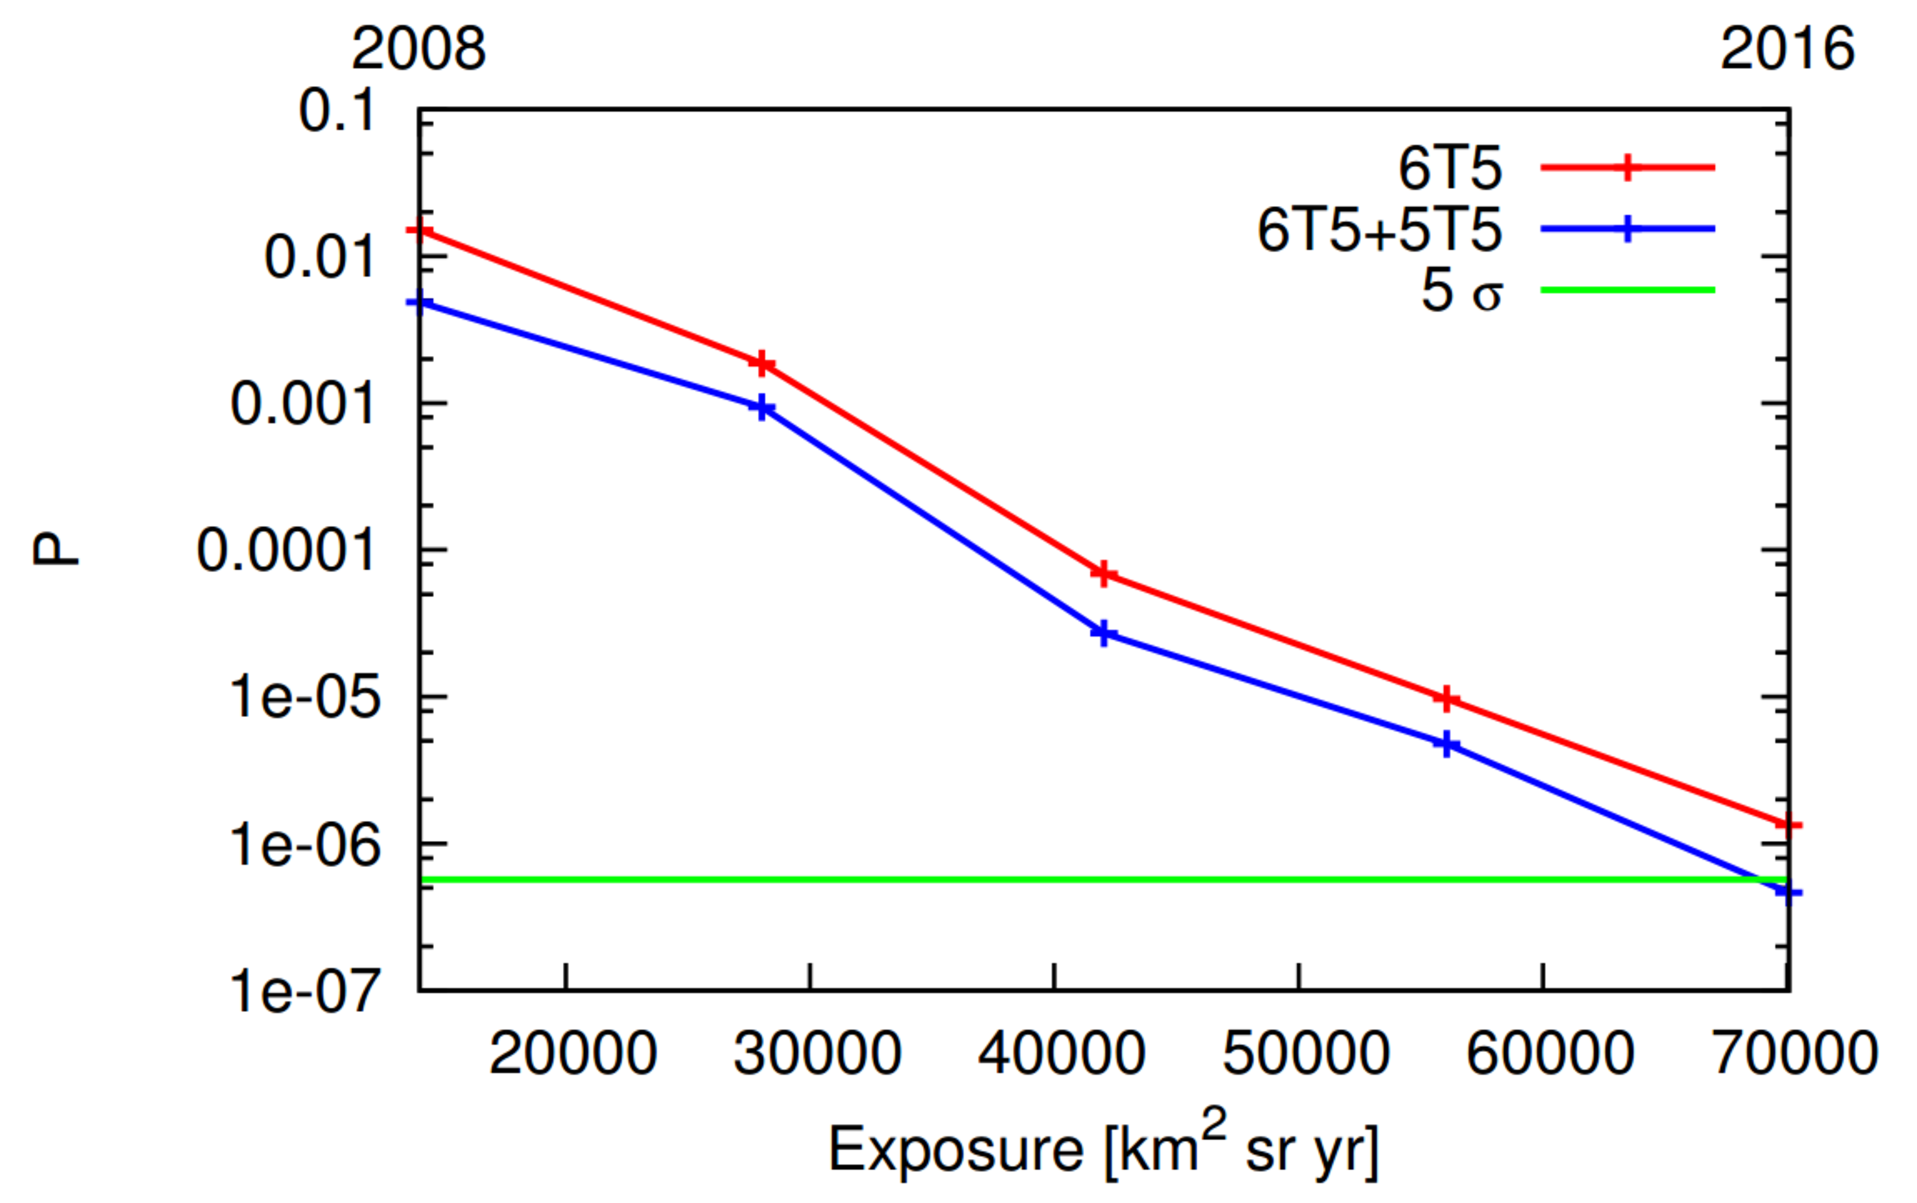
\includegraphics[height=5cm]{intro/auger_dipole_sig}
  \label{plot:pao_dipole_sig}}
  \caption[]{\subref{plot:pao_dipole} \subref{plot:pao_dipole_sig} Probability for the amplitude of the dipole to arise from an isotropic distribution as a function of the integrated exposure of the Pierre Auger Observatory. Various data sets with different tank triggers are shown \footnotemark \cite{Mollerach2016_1}.
  }
\label{fig:pao_dipole}
\end{figure}
\footnotetext{As discussed further in the reconstruction Chapter, quality cuts are performed on reconstructed data from the \ac{SD}. One of these cuts is known as the 6T5-trigger; it requires that the detector with the highest signal has all of its 6 closest neighbors working at the time of the event. Similarly, a 5T5 only requires 5 of the closest neighbors to be working.}
\end{lstlisting}



\section{Tables}

\begin{table}[h]
  \caption{Dipole components and direction in equatorial components \cite{Mollerach2016_2}.}
  \centering
  \begin{tabular}{cccccc}
  \toprule
  \textbf{$E$/EeV} & $\boldsymbol{d_\perp}$ & $\boldsymbol{d_z}$ & $\boldsymbol d$ & $\boldsymbol\alpha$ & $\boldsymbol\delta$  \\
  \midrule
  4-8 &  $-0.024 \pm 0.010$ & $ 0.006
   \pm 0.006$ & $0.025 \pm 0.009$ & \ang{-75} $\pm$ \ang{15} & \phantom{0}\ang{82} $\pm$ \ang{57}\\
   > 8 & $-0.026 \pm 0.015$ &  $0.060 \pm 0.010$ & $0.065 \pm 0.011$ & \ang{-24} $\pm$ \ang{12} & \ang{100} $\pm$ \ang{10}\\
  \bottomrule
  \end{tabular}
  \label{tb:pao_dipole}
\end{table}



\section{Mathematical and decay equations}

For decay equations, use align
%
\begin{align*}
  \gamma_\mathrm{CMB} + \mathrm{p} \rightarrow & \Delta^+ \rightarrow \mathrm{p} + \pi^0 \, ,\\
  \gamma_\mathrm{CMB} + \mathrm{p} \rightarrow & \Delta^+ \rightarrow \mathrm{n} + \pi^+ \, .
\end{align*}
\begin{lstlisting}
\begin{align*}
  \gamma_\mathrm{CMB} + p \rightarrow & \Delta^+ \rightarrow p + \pi^0 \, ,\\
  \gamma_\mathrm{CMB} + p \rightarrow & \Delta^+ \rightarrow n + \pi^+ \, .
\end{align*}
\end{lstlisting}

For writing \sig{5.5}, use
%
\begin{lstlisting}
\sig{5.5} 
\end{lstlisting}



\section{Reminders}

Use to dos so that you don't have to dig through latex code. [inline] makes it so it takes up the line and isn't hanging off the page
%
\begin{itemize}
\item To add a todo inline like this
\todo[inline]{more recent spectrum? proper citation to whom?} 
\begin{lstlisting}
\todo[inline]{more recent spectrum? proper citation to whom?} 
\end{lstlisting}
%
\item To generate this for missing figures:
\missingfigure{} % puts a giant yield sign and text describing what you want to add there
\begin{lstlisting}
\missingfigure{}
\end{lstlisting}
%
\item To generate a list of all your todos and their page numbers, use
\begin{lstlisting}
\listoftodos 
\end{lstlisting}
\end{itemize}



\section{Miscellaneous}

\begin{itemize}
\item  $4.6{\times}10^{-7}$
\begin{lstlisting}
$4.6{\times}10^{-7}$
\end{lstlisting}
\item For degrees \ang{148.4} 
\begin{lstlisting}
\ang{148.4} or 148.4^\circ
\end{lstlisting}
\item For formatting numbers otherwise in text, \num{-2.0}
\begin{lstlisting}
\num{-2.0} or $-2.0$
\end{lstlisting}
\item Superscripts for text like 20\textsuperscript{th}
\begin{lstlisting}
20\textsuperscript{th}
\end{lstlisting}
\item For marking out text ---\deleted{Due to the clean room environment}, use:
\begin{lstlisting}
\deleted{Due to the clean room environment}
\end{lstlisting}
This may be useful for editing your thesis later.
\end{itemize}
